\section{Entscheidungstabellen und -bäume}

\subsection{Einleitung}

Die Vorlesung "`Grundlagen des Entscheidens I"' hat das Ziel -- aus
philosophischer Perspektive -- in die Entscheidungs- und Spieltheorie
einzuführen. Dabei geht es vor allem um die Vermittlung von Grundlagen
und elementaren Lösungs- und Rechentechniken, d.h. wir werden
untersuchen, wie man Entscheidungsprobleme als Tabellen oder
Entscheidungsbäume darstellt, wie Entscheidungen unter Risiko (d.h.
bei bekannten Wahrscheinlichkeiten für das Eintreten unbeeinflussbarer
Ereignisse) und unter Unwissen (bei unbekannten Wahrscheinlichkeiten)
getroffen werden können, wie die strategische Interaktion zwischen
mehreren menschlichen Entscheidern mit Hilfe spieltheoretischer
Modelle dargestellt werden kann und vieles mehr. Dabei werden wir uns
immer auch mit den philosophischen Interpretationsfragen dieser
Techniken beschäftigen, sowie mit theoretischen Einwänden, von denen
es zahlreiche gibt.

Ausgespart bleibt in den "`Grundlagen des Entscheidens I"' jedoch
weitgehend die Frage der Anwendung dieser Theorie in verschiedenen
empirischen Wissenschaftsbereichen. Die Anwendbarkeit der Spiel- und
Entscheidungstheorie ist je nach Wissenschaftsbereich mehr oder
weniger stark umstritten. Während sie in der Ökonomie gewissermaßen
kanonisch ist, wird ihr Wert für die Sozial- und Politikwissenschaften
oft bestritten. Besonders die Veröffentlichung von Donald Greens und
Ian Shapiros Buch "`The Pathologies of Rational Choice"'
\cite{green-shapiro:1994}, ein Werk, das die Anwendung ökonomischer
Modelle im Bereich der Politikwissenschaften einer detaillierten und
präzisen Kritik unterzieht, hat eine sehr kontroverse Diskussion über
den Wert und Unwert des ökonomischen Theorieansatzes in den
Politikwissenschaften hervorgerufen. Wenn Zeit bleibt, werden wir am
Ende des Semesters an einem Beispiel untersuchen, worum es bei der
Kritik von Green und Shapiro geht, und aus welchen Gründen die
Anwendung der Spiel- und Entscheidungstheorie sowie das ihr zu Grunde
liegende "`Rational Choice"' Paradigma\footnote{Unter dem "`Rational
  Choice"' Paradigma wird hier die Auffassung verstanden, dass alle
  Menschen strikte Nutzenmaximierer sind, und dass sich sowohl das
  menschliche Handeln als auch gesellschaftliche Strukturen restlos
  und allein aus diesem Prinzip erklären lassen.} außerhalb des
engeren Kreises der Wirtschaftswissenschaften meist zum Scheitern
verurteilt ist.


\subsection{Der Gegenstand der Entscheidungstheorie}

Die Entscheidungstheorie, die in dieser Vorlesung vorgestellt wird,
ist eine
\marginline{Grund\-elemente:\\1.Zustände\\2.Handlungen\\3.Ergebnisse}
formale Theorie davon, wie man in Entscheidungssituationen
bestmögliche Entscheidungen trifft. Eine {\em Entscheidungssituation}
ist dabei charakterisiert durch 1) eine Menge von möglichen
(Welt-){\em Zuständen}, von denen wir entweder nicht wissen, in
welchem dieser möglichen Zustände sich die Welt tatsächlich befindet
(epistemische Unsicherheit), oder bei denen noch nicht feststeht,
welcher Zustand eintreten wird (reale Unsicherheit), 2) eine Menge von
{\em Handlungsalternativen} und 3) eine Menge von {\em Ergebnissen},
deren Realisierung von der gewählten Handlung und dem bestehenden
bzw. dem eingetretenen (Welt-)Zustand abhängt.

Kann man eine bestimmte Entscheidungssituation überhaupt in dieser Form
analysieren, dann lässt sich das Entscheidungsproblem sehr leicht schematisch
in einer Tabelle darstellen: 

\begin{center}
\begin{tabular}{cc|c|c|}
& \multicolumn{1}{c}{} & \multicolumn{2}{c}{{\bf Zustand}} \\
&                  & schwere Klausur   & leichte Klausur    \\ \cline{2-4}
& lernen           & {\em bestehen}    &  {\em bestehen}    \\ \cline{2-4}
\raisebox{1.5ex}[-1.5ex]{{\bf Handlung}} 
& schwimmen gehen  & {\em durchfallen} &  {\em bestehen} \\
\cline{2-4}
\end{tabular}
\end{center}

Die Zeilen repräsentieren in dieser Tabelle unterschiedliche
Handlungs\-alternativ\-en, die Spalten stellen die verschiedenen
Weltzustände dar. Die den Handlungen und Zuständen zugeordneten
Ergebnisse stehen in den entsprechenden Zeilen und Spalten innerhalb
der Tabelle. Diese Tabelle gibt natürlich nur ein äußerst einfaches
Entscheidungsproblem wieder. Ebensogut könnte man sich eine größere
Tabelle mit mehr Handlungsalternativen, z.B. "`lernen und
mitschreiben"', "`schwimmen gehen und mitschreiben"', "`krank
schreiben lassen"', oder mit mehr Zuständen, z.B. "`schwere"',
"`leichte"' und "`mittelschwere Klausur"', vorstellen.
 
Bei der Analyse realer Entscheidungsprobleme stellt es oft eine
Herausforderung \marginline{Das Problem der Problemspezifikation} dar,
alle Zustände und Handlungsalternativen zu identifizieren bzw. eine
geeignete Einteilung dafür zu finden.  Insbesondere dürfen sich die
Handlungsalterantiven untereinander (und ebenso die Zustände
untereinander) nicht überschneiden, das Ergebnis muss eindeutig von
den Handlungen abhängen und es sollten {\em alle} möglichen Zustände
berücksichtigt werden, die Einfluss auf das Ergebnis haben
können. Vergisst man irgendwelche Zustände, die Einfluss auf das
Ergebnis haben können, in der Entscheidungstabelle zu berücksichtigen,
so besteht die Gefahr, dass man unangenehme Überraschungen erlebt,
indem Ergebnisse eintreten, mit denen man nicht gerechnet
hat. Versäumt man umgekehrt, mögliche Handlungsalternativen zu
berücksichtigen, so schränkt man nur die eigene Entscheidungsfreiheit
unnötig ein, wird aber bei ansonsten korrekter Analyse keine
Überraschungen erleben. Mit diesen Schwierigkeiten, die die {\em
  Problemspezifikation} betreffen, werden wir uns in dieser
Vorlesungsreihe jedoch nur am Rande beschäftigen. Es sei jedoch darauf
hingewiesen, dass die korrekte Spezifikation des Entscheidungsproblems
eine hochgradig nicht-triviale Aufgabe sein kann, und dass die
praktische Anwendbarkeit der Entscheidungstheorie auch davon abhängig
ist, ob es in einer gegebenen Situation überhaupt möglich ist, eine
zuverlässige Problemspezifikation im Sinne der Entscheidungstheorie zu
geben.

Abgesehen von den Schwierigkeiten, die sich bei der
Problemspezifikation ergeben \marginline{Systematische Grenzen der
  Anwendbarkeit:} können, ist die Anwendbarkeit der
Entscheidungstheorie aber auch aus systematischen Gründen auf ganz
bestimmte Entscheidungsprobleme eingeschränkt. So kann sie uns
z.B. wenig weiterhelfen, wenn wir uns über die Ergebnisse bzw. die
Bewertung der Ergebnisse einer Entscheidungssituation selbst nicht im
Klaren sind.\marginline{1.Un\-ent\-schlossen\-heit hinsichtlich der
  Zielsetzung} Die Frage, ob jemand im Urlaub lieber ans Meer oder in
die Berge fahren will, stellt ganz sicher ein Entscheidungsprobem dar,
aber es handelt sich nicht um ein Entscheidungsproblem von der Sorte,
bei der uns die Entscheidungstheorie viel weiterhelfen kann. Vielmehr
handelt es sich um ein Problem, bei dem man sich über die eigenen
Präferenzen klar werden muss, man könnte auch sagen: um ein Problem,
bei dem man sich einfach entscheiden muss. In Anlehnung an bestimmte
Doktrinen in der Moralphilosophie bzw. in der politischen Philosophie
könnte man hier vielleicht von einem "`{\em dezisionistischen}
Entscheidungsproblem"' sprechen.

Weiterhin setzt die Entscheidungstheorie voraus, dass wir wissen,
welche möglichen Ergebnisse als Folge der von uns getroffenen
Entscheidungen überhaupt eintreten können.\marginline{2.Unwissenheit
  hinsichtlich der möglichen Ergebnisse} Es gibt aber viele
Situationen, in denen die möglichen Folgen unserer Handlungen für uns
schlicht unabsehbar sind. So können wir zwar absehen, dass sich der
$CO_2$ Gehalt in der Atmosphäre in Zukunft erhöhen wird, wenn wir die
Entscheidung treffen, den $CO_2$ Ausstoß nicht zu verringern, und mit
einer -- allerdings schon erheblich größeren Unsicherheit -- können
uns die Wissenschaftler sagen, dass sich dann das Klima erwärmen wird,
aber wie sich die Erwärmung und die daraus resultierenden klimatischen
Veränderungen gesellschaftlich und politisch auswirken werden, darüber
können wir nur spekulieren. Bei Entscheidungen, bei denen wir die
Menge der möglichen Ergebnisse nicht angeben können, weil wir es dabei
mit "`unknown unknowns"' zu tun haben, stehen wir mit der formalen
Entscheidungstheorie natürlich auf verlorenem Posten. In Bezug auf den
Klimawandel ist daher auch schon der Vorschlag gemacht worden statt
des auf der Entscheidungstheorie fußenden Utilitarismus, verstärkt
einen tugendethischen Ansatz in Anschlag zu bringen \cite[155ff.,
230ff.]{hillerbrand:2006}.\footnote{Da das Buch ansonsten sehr stark
  dem utilitaristischen Ansatz verpflichtet ist, vor allem auch gegen
  die nicht-anthropozentrische Naturethik etwa eines H. Jonas, wird
  man hinter diesem Vorschlag keine grundsätzliche Ablehnung des
  Utilitarismus oder wissenschaftliche Unbedarftheit vermuten dürfen.}

Damit scheiden neben den Entscheidungsproblemen, die aus praktischen
Gründen keine adäquate Problemspezifikation zulassen, viele weitere
wichtige Enscheidungsprobleme aus dem Anwendungsbereich der formalen
Entscheidungstheorie schon von vornherein aus. Es ist wichtig sich
diesen Sachverhalt, dass die Entscheidungstheorie nur einen Teil der
realen Entscheidungsprobleme adäquat behandeln kann, vor Augen zu
halten. Denn dies bedeutet, dass die Entscheidungstheorie, die wir
hier besprechen, nicht notwendigerweise die Theorie der Entscheidungen
schlechthin ist. Oft ist es der Fall, dass wir diejenigen
Entscheidungsprobleme, für die diese Theorie ungeeignet ist, immer
noch im Rahmen anderer, von ihrem Stil her vielleicht ganz
andersartiger Theorien und Ansätze behandeln können, so wie für die
Ethik des Klimaschutzes eine Tugendethik vorgeschlagen worden ist, um
den Schwierigkeiten des Utilitarismus angesichts extremer Unsicherheit
("`unknown unknowns"') zu begegnen.

\marginline{Nachteile des methodenzentrierten Ansatzes} In noch einmal
verschärfter Form stellt sich dasselbe Problem für die Spieltheorie,
deren empirische Anwendungsfälle außerhalb der Ökonomie eher dünn
gesät sind. Die Gefahr besteht daher, dass man durch die einseitige
Konzentration auf solche Probleme, die sich mit Hilfe derartiger
Theorien methodisch in den Griff bekommen lassen, ein völlig falsches
Bild von dem emprischen Sachbereich bekommt, auf den sie sich
beziehen, und von dem sie nur einen kleinen Ausschnitt erfassen
können, der in Wahrheit aber größtenteils ganz anderen Gesetzen
gehorcht. Dass diese Gefahr vornehmlich bei szientistischen, d.h. sich
strenger und formaler Methoden nach dem Vorbild der
Naturwissenschaften bedienender Ansätze auftritt, hängt mit der
Methodenzentriertheit dieser Ansätze zusammen, die dazu führt, dass
vornehmlich solche Probleme als wissenschaftlich relevant ausgewählt
und der Untersuchung für wert befunden werden, die zum vorgegebenen
Methodenkanon passen, anstatt umgekehrt zu gegebenen empirischen
Problemen und Fragestellungen die zur ihrer Behandlung geeigneten
Methoden auszuwählen. A priori sind übrigens der methodenzentrierte
Ansatz und sein Gegenstück, der problemorientierte Ansatz,
gleichermaßen legitim. Nur ist die Gefahr der intellektuellen
Selbsttäuschung beim methodenzentrierten Ansatz offenbar erheblich
größer und tritt daher genau da auf, wo wir sie am wenigsten erwarten
würden, nämlich dort, wo auch das Bewusstsein wissenschaftlicher
Strenge am größten ist.\footnote{Siehe dazu die Kritik von Ian Shapiro
  \cite{shapiro:2005} oder von John Dupré \cite{dupre:2001}, sowie die
  ausführliche Studie von Donald Green und Ian Shapiro
  \cite{green-shapiro:1994}. Besonders das letztere Buch hat eine rege
  Diskussion hervorgerufen. Eine Verteidigung des formalen Rational
  Choice Ansatzes gegen die Kritik von Green und Shapiro hat neben
  anderen Gary W. Cox\cite{cox:1999} unternommen. Cox Ansicht
  allerdings, dass man selbst dann noch theoretische Erfolge für eine
  Theorie reklamieren kann, wenn sie empirisch erfolglos ist
  \cite[S.159-164]{cox:1999}, geht an dem grundlegenden Ziel der
  Wissenschaft vorbei, das selbstverständlich in der Erklärung von
  Vorgängen in der empirischen Welt besteht und nichts anderem, und
  ist eher ein Beispiel wie Wissenschaftlicher sich lieber die
  Wissenschaftstheorie zurechtbiegen als ein Scheitern des von ihnen
  verfolgten Ansatzes einzugestehen. Eine wissenschaftliche Theorie,
  die falsch ist, oder deren Richtigkeit oder Falschheit man nicht
  empirisch feststellen kann, kann man unmöglich "`erfolgreich"'
  nennen.}

Immerhin verbleiben der formalen Entscheidungstheorie aber weite
Bereiche, innerhalb derer wir sie fruchtbar und gewinnbringend
anwenden können. (Und dort wo man sie anwenden kann, ist man mit Hilfe
der Theorie anderen, intuitiven Entscheidungsfindungsmechanismen so
gut wie immer überlegen!) Sofern die Menge der möglichen Ergebnisse
und die Menge der Zustände bekannt ist, können wir sie selbst dann
noch heranziehen, wenn wir nicht einmal wissen, mit welcher
Wahrscheinlichkeit wir mit einem bestimmten Zustand rechnen müssen. In
diesem Fall handelt es sich um "`Entscheidungen unter Unwissen"'. Den
dazugehörigen Teil der Entscheidungstheorie werden wir in der nächsten
und übernächsten Woche besprechen. Sind die Wahrscheinlichkeiten, mit
denen bestimmte Ereignisse eintreten können, dagegen bekannt, dann
spricht man von "`Entscheidungen unter Risiko"'. In diesem Fall lässt
sich die Entscheidungstheorie sogar noch viel besser anwenden, was in
den darauf\/folgenden Wochen demonstriert wird. Was schließlich die
Spieltheorie, die wir als Letztes in diesem Semester ansprechen
werden, von der Entscheidungstheorie unterscheidet, ist, dass sie die
strategische Interaktion zwischen mehreren Entscheidern ("`Spielern"')
untersucht, die wechselseitig aufeinander reagieren bzw. die Reaktion
des Gegenübers antezipieren können. An die Stelle der (Welt-)Zustände
in der Entscheidungstheorie treten in der Spieltheorie also die Züge
des anderen Spielers.

\subsection{Darstellungsformen}

Zum Abschuss dieser Vorlesungsstunde soll -- sozusagen als
"`Appetizer"' -- wenigstens schon ein kurzer Einblick in die
Entscheidungstheorie selbst gegeben werden, mit der wir uns im Laufe
des Semesters eingehend beschäftigen werden. Wir werden im folgenden
Entscheidungsbäume und Entscheidungstabellen als zwei unterschiedliche
Formen der Darstellung von Entscheidungsproblemen kennen lernen und
zeigen, dass sich beide Darstellungsformen wechselseitig ineinander
überführen lassen.

\subsubsection{Entscheidungsbäume und -tabellen}

Zuvor hatten wir schon ein einfaches Beispiel einer
Entscheidungstabelle angeführt. Dies ist nicht die einzige Form, in
der man Entscheidungsprobleme schematisch darstellen kann. Eine
andere, wahrscheinlich sogar anschaulichere Form der schematischen
Darstellung ist der {\em Entscheidungsbaum}. Die weiter oben schon
einmal als Entscheidungstabelle dargestellte Entscheidungssituation
sieht als Baum folgendermaßen aus:

\begin{center} 
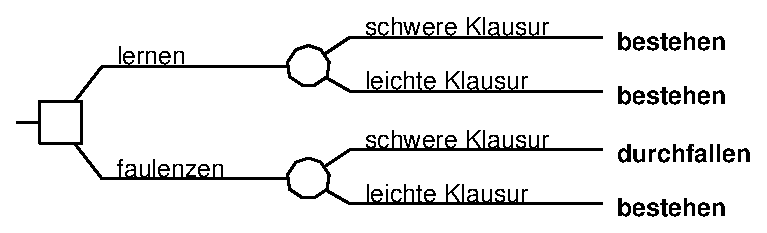
\includegraphics[width=12cm]{Grafiken/Beispiel1_1.eps}
\end{center}

Entscheidungsbäume bestehen immer aus Knoten und Ästen.
\marginline{Entscheidungs\-knoten\\~\\ und\\~\\
  Möglich\-keits\-knoten} Dabei werden die\-jenigen Knoten, an denen
eine Entscheidung zwischen unterschiedlichen Handlungsalternativen
getroffen werden muss, {\em Entscheidungs\-knoten}
genannt. Entscheidungsknoten werden durch ein Quadrat
symbolisiert. Diejenigen Knoten, die ein Zufallsereigniss
repräsentieren, werden {\em Möglichkeits\-knoten} genannt und durch
einen Kreis symbolisiert. Eingangs wurde statt von
"`Zufallsereignissen"' von "`Zuständen"' gesprochen. Die Zweige, die
auf einen Entscheidungsknoten folgen, stellen dabei unterschiedliche
"`Handlungsalternativen"' dar, zwischen denen die Entscheiderin wählen
kann.  Die Zweige, die auf einen Möglichkeitsknoten folgen,
entsprechen dagegen unterschiedlichen (Welt)-"'Zuständen"', von denen
entweder nicht sicher ist, welcher davon eintreten wird, oder von
denen wir nicht wissen welcher eintreten wird oder bereits eingetreten
ist, so dass es sich aus Sicht des Entscheiders immer noch um ein
zufälliges Ereignis handelt. (Die Unterscheidung zwischen
epistemischer Unsicherheit und objektiver Unbestimmtheit und, damit
einhergehend, die zwischen subjektiver und objektiver
Wahrscheinlichkeit muss uns an dieser Stelle noch nicht
interessieren.) Die Ergebnisse stehen am Ende der Äste.

\marginline{Umwandlung von Tabellen in Bäume} Hat man eine
Entscheidungssituation, wie in diesem Fall, bereits durch eine
Entscheidungstabelle dargestellt, dann kann man daraus sehr einfach
einen Entscheidungsbaum ableiten, der dieselbe Entscheidungssituation
wiedergibt: Man beginnt mit einem viereckigen Entscheidungsknoten. An
diesen Entscheidungsknoten hängt man alle Handlungsalternativen an,
die in der ersten Spalte der Tabelle stehen. Jeder dieser Zweige wird
dann mit einem runden Möglichkeitsknoten versehen, an den wiederum
alle Zustände angehängt werden, die in der ersten Zeile der Tabelle
stehen. Am Ende der Zweige wird dann das jeweilige Ergebnis aus der
Tabelle eingetragen.

Entscheidungsbäume haben gegenüber Entscheidungstabllen den Vorteil
größerer Anschaulichkeit. Umgekehrt erlauben Tabellen eine kompaktere
Darstellung. Die größere Anschaulichkeit soll an einem weiteren
Beispiel demonstriert werden.  Bei diesem Beispiel geht es um eine
Person, die vor der Entscheidung steht, ob sie an einem Sonntag bei
unsicherer Wetterprognose zur Küste fahren und sich dort entweder
sonnen oder, falls es regnet, dort angeln gehen würde. Die
Entscheidungssituation, die mehrere Einzelentscheidungen beinhaltet
(1) zur Küste fahren oder nicht, 2) bei Regen: Angeln gehen oder
gleich heimkehren) könnte folgendermaßen aussehen:

\begin{center}
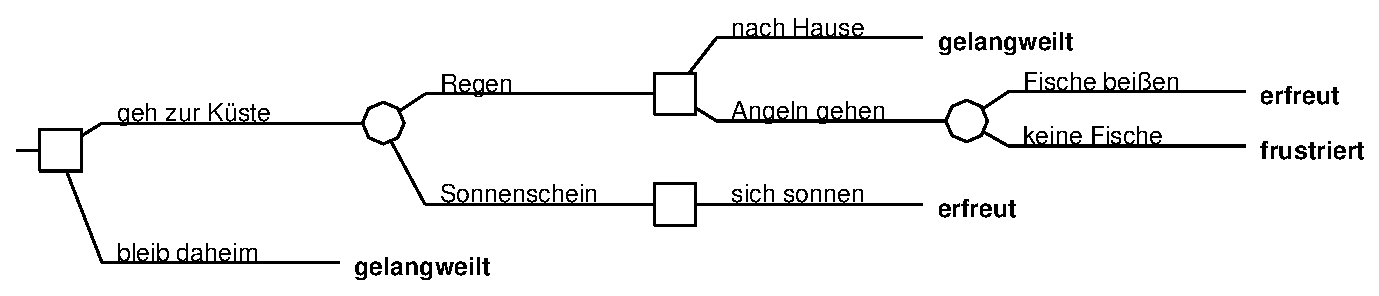
\includegraphics[width=12cm]{Grafiken/Beispiel1_2.eps}
\end{center}
(Beispiel aus \cite[S. 18]{resnik:1987})

Entscheidungsbäume erlauben es komplexe Entscheidungen, die aus
mehreren Einzelentscheidungen zusammengesetzt sind, in ihrem Verlauf
darzustellen.  Dennnoch kann man jedes Entscheidungsproblem, dass sich
durch einen Entscheidungsbaum beschreiben lässt auch als
Entscheidungstabelle darstellen.  Dazu muss man die möglichen
Sequenzen von Einzelentscheidungen zu {\em Gesamtstrategien}
zusammenfassen. Solche Gesamtstrategien müssen die "`unter allen
möglichen Eventualitäten"' zu treffenden Einzelentscheidungen
festlegen.  Gleichfalls ist es meist erforderlich, die
Zufallsereignisse zu komplexeren Zuständen zusammenzufassen. Verfährt
man in dieser Weise, dann entsteht aus dem eben präsentierten
Entscheidungsbaum folgende Tabelle:

\begin{center}
\label{AngelnBeispiel}
\begin{tabular}{c|c|c|c|}
\multicolumn{1}{c}{}  & \multicolumn{1}{c}{Regen und Fische beißen}  & \multicolumn{1}{c}{Regen und keine Fische}  & \multicolumn{1}{c}{Sonnenschein} \\ \cline{2-4}
 A1 & gelangweilt & gelangweilt & erfreut \\ \cline{2-4}
 A2 & erfreut & frustriert & erfreut \\ \cline{2-4}
 A3 & gelangweilt & gelangweilt & gelangweilt \\ \cline{2-4}
\end{tabular}
\begin{itemize}
\item {\em A1}: geh zur Küste;  wenn Regen dann nach Hause,  sonst wenn Sonnenschein dann sich sonnen
\item {\em A2}: geh zur Küste;  wenn Regen dann Angeln gehen,  sonst wenn Sonnenschein dann sich sonnen
\item {\em A3}: bleib daheim
\end{itemize}

\end{center}

\begin{quotation}
\begin{small}
{\em Quizfrage: Kann man anhand dieser Entscheidungstabelle 
 bereits feststellen, welche 
Handlungsalternative gewählt werden
sollte oder zumindest sagen, ob eine bestimmte
Handlungsalternative definitiv nicht gewählt werden sollte?}
\end{small}
\end{quotation}

Nehmen Sie sich ruhig ein wenig Zeit, um sich klar zu machen, dass die
Tabelle dem Entscheidungsbaum entspricht, d.h. dass alle
Handlungsalternativen, die nach der Baumdarstellung gewählt werden
können, auch nach der Tabellendarstellung möglich sind, und ebenso
auch alle denkbaren Kombinationen von Zufallsereignissen. Man könnte
sich dabei zunächst wundern, warum beispielsweise die Kombination der
Ereignisse "`Sonnenschein"' und "`Fische beißen"' nicht in der Tabelle
vorkommt. Aber da in dem Fall, dass die Sonne scheint, der zweite
Möglichkeitsknoten gar nicht mehr erreicht wird, wirkt sich der
Unterschied, ob die Fische beißen oder nicht, auch nicht auf das
Ergebnis aus. Insofern können beide Fälle durch ein- und dieselbe
Zustandsspalte "`Sonnenschein"' erfasst werden

Das Verfahren, wie man einen Entscheidungsbaum in eine Tabelle
überführt, ist ebenfalls rein mechanischer Art. Da es etwas
komplizierter ist als die Umwandlung einer Tabelle in einen
Entscheidungsbaum, werden wir es gleich (Abschnitt \ref{BaumTabelle})
ausführlicher betrachten. Bis dahin soll einfach als gegeben
angenommen werden, dass dies immer möglich ist.

% Die Einzelheiten dieses Verfahrens, das intuitiv sehr
% viel leichter zu erfassen als exakt zu beschreiben ist, müssen uns an dieser
% Stelle nicht interessieren. Ebenso soll an dieser Stelle der Beweis, dass sich
% jeder Entscheidungsbaum in eine Tabelle, die dasselbe Entscheidungsproblem
% ausdrückt, überführen lässt, übergangen werden. (Der Beweis besteht im
% wesentlichen darin, ein Verfahren zur Transformation eines Entscheidungsbaums
% in eine Tabelle anzugeben. Dieser Beweis erfordert keine besonders originellen
% Ideen. Die Kunst besteht jedoch darin, das entsprechende Verfahren exakt zu
% beschreiben; so exakt, dass man es in einen Computer einprogrammieren könnte.
% Wer möchte kann sich ja mal daran versuchen ;) )

Wenn wir es aber einmal als gegeben betrachten, dass man jeden
Entscheidungsbaum in eine Entscheidungstabelle überführen kann, und,
wie zuvor schon gezeigt wurde, jede Entscheidugnstabelle in einen
Entscheidungsbaum, dann hat das die für uns wichtige Konsequenz, dass
wir frei sind, uns je nach Konvenienz der einen oder der anderen
Darstellung zu bedienen. Dies gilt insbesondere für die Entwicklung
der Entscheidungstheorie selbst. Denn wir können nun davon ausgehen,
dass alle Überlegungen, die wir in Bezug auf Entscheidungsprobleme
anhand einer der Darstellungsformen anstellen, ihre Gültigkeit
behalten, wenn wir zu der anderen Darstellungsform übergehen. Für die
Entwicklung der Theorie eignet sich dabei die kompaktere Tabellenform
häufig besser. Umgekehrt bietet sich für die Darstellung und Lösung
bestimmter Entscheidungsprobleme oft eher die anschaulichere
Darstellung durch Entscheidungsbäume eher an.

Wenn die Rede davon war, dass sich Tabellendarstellung und
Baumdarstellung auf mechanische Weise ineinander überführen lassen, so
bedeutet das allerdings nicht, dass wenn man nach diesem Verfahren
einen Entscheidungsbaum zuerst in eine Tabelle und dann wieder in
einen Baum überführt, auch derselbe Entscheidungsbaum wieder dabei
heraus kommt. Transformiert man die eben gewonnene Tabelle wieder in
einen Baum, so hat dieser Entscheidungsbaum die folgende Gestalt:

\begin{center}
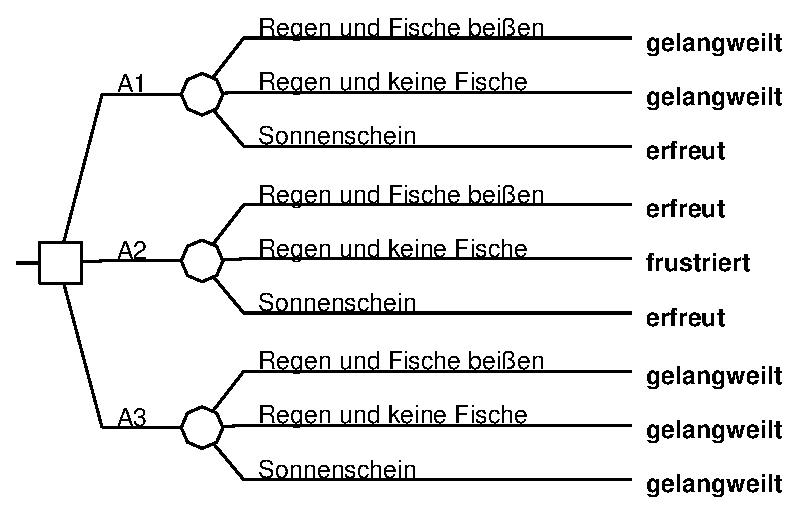
\includegraphics[width=12cm]{Grafiken/Beispiel1_4.eps}
\end{center}

Dass der Entscheidungsbaum nach der Übertragung in die Tabellenform und dann
wieder der Rückübertragung in die Baumform ganz anders aussieht, sollte
allerdings nicht verwundern, denn es gibt in der Regel viele unterschiedliche 
Möglichkeiten ein- und dasselbe Entscheidungsproblem als Baum- und Tabelle
darzustellen. Der zuletzt gezeigte Baum stellt in der Tat dasselbe
Entscheidungsproblem dar wie der ursprüngliche Baum. Identisch sind zwei
Entscheidungsprobleme genau dann, wenn denselben Kombinationen von
Handlungsalternativen und Zuständen dieselben Ergebnisse zugeordnet sind. Bei
Entscheidungen unter Risiko müssen die möglichen Weltzustände darüber hinaus
mit denselben Wahrscheinlichkeiten eintreten. Leider kann man weder der
Baumdarstellung noch der Tabellendarstellung unmittelbar ansehen, ob zwei
Entscheidungsprobleme identisch sind. Für die Entscheidungsbäume ist dies nach
dem vorhergehenden Beispiel offensichtlich. Bei Tabellen ergibt sich dies unter
anderem daraus, dass die Reihenfolge der Spalten und Zeilen für das zu Grunde
liegende Entscheidungsproblem egal ist (siehe Aufgabe
\ref{ZeilenSpaltenPermutation}).


\subsubsection{Exkurs: Entscheidungsbäume in Tabellen umwandeln}
\label{BaumTabelle}

{\em Dieses Teilkapitel ist als Exkurs gedacht. Wem es für den Anfang zu
schwierig ist, der kann diesen Exkurs (und die dazu gehörigen Übungsaufgaben) 
ruhig überspringen. Im Folgenden wird darauf nicht mehr zurück gegriffen.}

Um Entscheidungsbäume in Tabellen umzuwandeln, können wir uns den
Umstand zu Nutze machen, dass Entscheidungsbäume, so kompliziert sie
auch sein mögen, aus der Kombination von nur zwei Elementen bestehen,
Entscheidungsknoten und Zufallsknoten. Um einen Entscheidungsbaum in
eine Tabelle zu überführen müssen wir also nur wissen, wie man 1)
Entscheidungsknoten in eine Tabelle überträgt, wie man 2)
Zufallsknoten in eine Tabelle überträgt und 3) wie man einen
komplizierten zusammengesetzten Baum schrittweise mit Hilfe der beiden
vorherigen Übertragungsregeln reduziert.

1) Ein Entscheidungsbaum, der nur aus einem einzigen Ent\-scheidungs\-knoten mit
zwei Alternativen besteht, ergibt eine Tabelle mit zwei Zeilen und einer Spalte:

\vspace{0.5cm}

\parbox{7cm}{Baum:}\parbox{5cm}{Tabelle:}

\vspace{0.25cm}

\parbox{7cm}{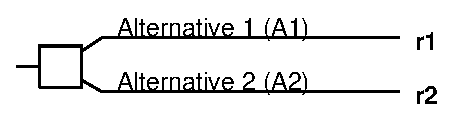
\includegraphics[width=6cm]{Grafiken/Beispiel1b_1.eps}}
\parbox{5cm}{
\begin{tabular}{c|c|}
      & $S_1$ \\ \cline{1-2}
$A_1$ & $r_1$ \\ \cline{1-2}
$A_2$ & $r_2$ \\ \cline{1-2}
\end{tabular}}

\vspace{0.5cm}

2) Ein Baum, der nur aus einem Zufallsknoten besteht, liefert demgegenüber eine
Tabelle mit nur einer Zeile und genau soviel Spalten wie Ereignisse an dem
entsprechenden Ereignisknoten eintreten können.

\vspace{0.5cm}

\parbox{7cm}{Baum:}\parbox{5cm}{Tabelle:}

\vspace{0.25cm}

\parbox{7cm}{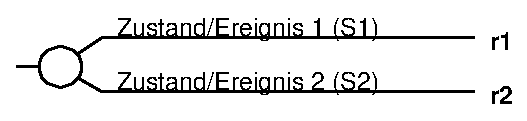
\includegraphics[width=6cm]{Grafiken/Beispiel1b_2.eps}}
\parbox{5cm}{
\begin{tabular}{c|c|c|}
      & $S_1$ & $S_2$ \\ \cline{1-3}
$A_1$ & $r_1$ & $r_2$ \\ \cline{1-3}
\end{tabular}}

\vspace{0.5cm}

3) Wie kann man nun aber einen Entscheidungsbaum, der aus einer
Vielzahl von Entscheidungs- und Zufallsknoten besteht, in eine Tabelle
überführen? Dazu wird der Baum schrittweise von hinten
"`aufgerollt"'. Die jeweils "`letzten"' Entscheidungs-
bzw. Zufallsknoten von rechts entsprechen genau den vorher
beschriebenen Fällen und können auf die beschriebende Weise
umgewandelt werden.  Kompliziert wird es erst bei den weiter in der
Mitte und am Anfang liegenden Knoten. Wenn wir an einem solchen Knoten
ankommen, haben wir den Baum aber schon soweit aufgerollt, dass wir zu
den sich an den Knoten anschließenden Teilbäumen bereits über Tabellen
verfügen. Das Problem stellt sich also folgendermaßen dar: Wie kann
ein Entscheidungsknoten bzw. ein Zufallsknoten in eine Tabelle
überführt werden, an dessen Enden sich wiederum ganze
Entscheidungsbäume anschließen, für die wir aber immerhin schon über
eine Repräsentation in Tabellenform verfügen?

Um dieses Problem zu lösen, müssen wir wiederum Entscheidungs- und
Zufallsknoten getrennt betrachten:

3 a) Angenommen, wir haben es mit einem Entscheidungsknoten zu tun. Dann endet
der Entscheidungsknoten in zwei Teilbäumen, die bereits als Tabellen
dargestellt sind. Jede dieser Tabellen enthält wiederum eine Menge von
Handlungsalternativen und eine Menge von Zufallsereignissen.

\vspace{0.5cm}

\begin{small}
\parbox{3.5cm}{\ }
\parbox{4.5cm}{\begin{center}Tabelle zu Baum 1\end{center}}
\parbox{4.5cm}{\begin{center}Tabelle zu Baum 2\end{center}}

\parbox{3.5cm}{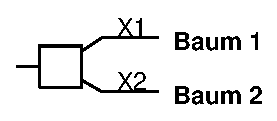
\includegraphics[width=3.5cm]{Grafiken/Beispiel1b_3.eps}}
\parbox{4.5cm}{
\begin{tabular}{c|ccc|}
         & $S_1$    & $\cdots$ & $S_n$     \\ \cline{1-4}
$A_1$    & $r_{11}$ & $\cdots$ & $r_{1n}$  \\ %\cline{1-4}
$\vdots$ & $\vdots$ & $\ddots$ & $\vdots$  \\ %\cline{1-4}
$A_m$    & $r_{m1}$ & $\cdots$ & $r_{mn}$  \\ \cline{1-4}
\end{tabular}}
\parbox{4.5cm}{
\begin{tabular}{c|ccc|}
         & $T_1$    & $\cdots$ & $T_l$     \\ \cline{1-4}
$B_1$    & $u_{11}$ & $\cdots$ & $u_{1l}$  \\ %\cline{1-4}
$\vdots$ & $\vdots$ & $\ddots$ & $\vdots$  \\ %\cline{1-4}
$B_h$    & $u_{h1}$ & $\cdots$ & $u_{hl}$  \\ \cline{1-4}
\end{tabular}}
\end{small}

\vspace{0.5cm}

Die beiden Ereignismengen $\{S_1, \ldots, S_n\}$ und $\{T_1, \ldots, T_l\}$ des
ersten und des zweiten Teilbaums sowie die entsprechenden Mengen von
Handlungsalternativen $\{A_1, \ldots, A_m\}$ und $\{B_1, \ldots, B_h\}$ müssen
nun in geeigneter Form kobminiert werden, um die Tabelle des gesamten
Entscheidungsknotens aufzubauen. Das geschieht folgendermaßen: In den Spalten
der zusammengefassten Tabelle muss jede mögliche Kombination der
Zufallsereignisse aus beiden Mengen eingetragen werden. In den Zeilen wird als
erstes der Block von Handlungen $X_1 \wedge A_1,\ldots, X_1 \wedge A_m$
eingetragen, worauf als zweites ein Block von Handlungen $X_2 \wedge
B_1,\ldots, X_2 \wedge B_h$ folgt (d.h. jede der Handlungen der ersten Tabelle
wird mit der Handlung $X_1$ kombiniert, jede alternative Handlung der zweiten
Tabelle mit $X_2$).\footnote{Das aus der Logik bekannte Zeichen $\wedge$
bedeutet "`und"', so dass der Ausdruck $X_1 \wedge A_1$ so zu verstehen ist,
dass die Handlung $X_1$ {\em und} die (möglicherweise wiederum aus mehreren
Einzelhandlungen zusammengesetzte) Handlung $A_1$ ausgeführt werden.} Daraus
ergibt sich folgende kombinierte Tabelle:

\begin{small}
\begin{center}
\begin{tabular}{c|ccc|c|ccc|}
                 & $S_1 \wedge T_1$  & $\cdots$ & $S_n \wedge T_1$ & $\cdots$
                 & $S_1 \wedge T_l$  & $\cdots$ & $S_n \wedge T_l$  
                 \\ \cline{1-8} 
$X_1 \wedge A_1$ & $r_{11}$          & $\cdots$ & $r_{1n}$ & $\cdots$ 
                 & $r_{11}$          & $\cdots$ & $r_{1n}$  \\
  $\vdots$       & $\vdots$          & $\ddots$ & $\vdots$ & $\ddots$
                 & $\vdots$          & $\ddots$ & $\vdots$\\
$X_1 \wedge A_m$ & $r_{m1}$          & $\cdots$ & $r_{mn}$ & $\cdots$
                 & $r_{m1}$          & $\cdots$ & $r_{mn}$\\ \cline{1-8}
                   
$X_2 \wedge B_1$ & $u_{11}$          & $\cdots$ & $u_{11}$ & $\cdots$
                 & $u_{1l}$          & $\cdots$ & $u_{1l}$\\
  $\vdots$       & $\vdots$          & $\ddots$ & $\vdots$ & $\ddots$
                 & $\vdots$          & $\ddots$ & $\vdots$\\                  
$X_2 \wedge B_h$ & $u_{h1}$          & $\cdots$ & $u_{h1}$ & $\cdots$
                 & $u_{hl}$          & $\cdots$ & $u_{hl}$\\\cline{1-8}
\end{tabular}
\end{center}
\end{small}

Man beachte: Jedes mögliche Resultat $r_{xy}$ aus der ersten Tabelle kommt genau
$l$-mal vor, d.h. genauso viel mal, wie es Zufallsereignisse in der zweiten
Tabelle gibt. Umgekehrt kommt jedes mögliche Resultat $u_{xy}$ aus der zweiten Tabelle
genau $n$-mal vor, wobei $n$ die Anzahl der Zufallsereignisse in der
ersten Tabelle ist. (Die entsprechende Tabellendarstellung ist also in
der Regel hochgradig redundant und könnte, wenn dies der Fall ist, nachträglich
noch vereinfacht werden.)

\vspace{0.5cm}

3 b) Geht es statt dessen um die Umwandlung eines Zufallsknotens, dann stehen
wir vor der spiegelbildlichen Situation, so dass wir diesmal zwei Spaltenblöcke
bilden und in den Zeilen jede Kombination möglicher Handlungen zu
berücksichtigen haben. 

\vspace{0.5cm}

\begin{small}
\parbox{3.5cm}{\ }
\parbox{4.5cm}{\begin{center}Tabelle zu Baum 1\end{center}}
\parbox{4.5cm}{\begin{center}Tabelle zu Baum 2\end{center}}

\parbox{3.5cm}{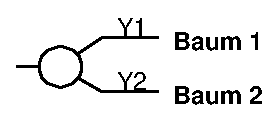
\includegraphics[width=3.5cm]{Grafiken/Beispiel1b_4.eps}}
\parbox{4.5cm}{
\begin{tabular}{c|ccc|}
         & $S_1$    & $\cdots$ & $S_n$     \\ \cline{1-4}
$A_1$    & $r_{11}$ & $\cdots$ & $r_{1n}$  \\ %\cline{1-4}
$\vdots$ & $\vdots$ & $\ddots$ & $\vdots$  \\ %\cline{1-4}
$A_m$    & $r_{m1}$ & $\cdots$ & $r_{mn}$  \\ \cline{1-4}
\end{tabular}}
\parbox{4.5cm}{
\begin{tabular}{c|ccc|}
         & $T_1$    & $\cdots$ & $T_l$     \\ \cline{1-4}
$B_1$    & $u_{11}$ & $\cdots$ & $u_{1l}$  \\ %\cline{1-4}
$\vdots$ & $\vdots$ & $\ddots$ & $\vdots$  \\ %\cline{1-4}
$B_h$    & $u_{h1}$ & $\cdots$ & $u_{hl}$  \\ \cline{1-4}
\end{tabular}}
\end{small}

\vspace{0.5cm}

Um die kombinierte Tabelle zu konstruieren, müssen wir also zwei Spaltenblöcke
bilden, wobei der erste Block alle Zufallsereignisse der ersten Tabelle umfasst
(und-verknüpft mit dem Ereignis $Y_1$ versteht sich!) und der zweite Block die
der zweiten Tabelle: In den Zeilen treten alle Kombinationen möglicher
Handlungen auf, und zwar, da die Möglichkeit, eine bestimmte Handlung zu
wählen oder nicht zu wählen erst durch das Eintreten von $Y_1$ oder $Y_2$
überhaupt eröffnet wird, in einer "`wenn\ldots, dann\ldots"'-Form. In einer 
abgekürzten Schreibweise, bei der das Zeichen "`$\rightarrow$"' für die 
wenn-dann-Beziehung stehen soll, schreiben wir also z.B.
$(Y_1 \rightarrow A_2) \wedge (Y_2 \rightarrow B_5)$.\footnote{Angesichts der 
Symmetrie zwischen dem Problem der Umwandlung eines Entscheidungsknotens 
in eine Tabelle und dem der Umwandlung eines
Zufallsknotens in eine Tabelle, könnte es verwundern, dass wir im zweiten Fall
in den Zeilen der generierten Tabelle "`wenn\ldots, dann\ldots"'-Audrücke
vorfinden, während wir uns im ersteren Fall mit simpleren und-Verknüpfungen
begnügen. Dies ist dadurch motiviert, dass wir davon ausgehen, dass die
Ereignisse der Serien $T_1, \ldots, T_n$ bzw. $S_1, \ldots, S_n$ unabhängig von
den getroffenen Entscheidungen auch dann eintreten, wenn sie angesichts des gewählten Zweiges
für das erzielbare Ergebnis nicht mehr relevant sind. Diese Annahme ist
zwar harmlos aber keinesfalls zwingend. Wollte man ganz präzise sein, dann
müsste man die Spaltenüberschriften der aus einem Entscheidungsknoten gewonnen Tabelle
ebenfalls als "`wenn\ldots, dann\ldots"'-Aussagen ausformulieren.}

\begin{small}
\begin{center}
\begin{tabular}{c|ccc|ccc|}
                 & $Y_1 \wedge S_1$  & $\cdots$ & $Y_1 \wedge S_n$
                 & $Y_2 \wedge T_1$  & $\cdots$ & $Y_2 \wedge T_l$  
                 \\ \cline{1-7} 
$Y_1 \rightarrow A_1 \wedge Y_2 \rightarrow B_1$  
                 & $r_{11}$          & $\cdots$ & $r_{1n}$  
                 & $u_{11}$          & $\cdots$ & $u_{1l}$  \\
  $\vdots$       & $\vdots$          & $\ddots$ & $\vdots$ 
                 & $\vdots$          & $\ddots$ & $\vdots$\\
$Y_1 \rightarrow A_1 \wedge Y_2 \rightarrow B_h$     
                 & $r_{11}$          & $\cdots$ & $r_{1n}$ 
                 & $u_{h1}$          & $\cdots$ & $r_{hl}$\\ \cline{1-7}

  $\vdots$       & $\vdots$          & $\ddots$ & $\vdots$ 
                 & $\vdots$          & $\ddots$ & $\vdots$\\ \cline{1-7}
                   
$Y_1 \rightarrow A_m \wedge Y_2 \rightarrow B_1$  
                 & $r_{m1}$          & $\cdots$ & $r_{mn}$  
                 & $u_{11}$          & $\cdots$ & $u_{1l}$  \\
  $\vdots$       & $\vdots$          & $\ddots$ & $\vdots$ 
                 & $\vdots$          & $\ddots$ & $\vdots$\\
$Y_1 \rightarrow A_m \wedge Y_2 \rightarrow B_h$     
                 & $r_{m1}$          & $\cdots$ & $r_{mn}$ 
                 & $u_{h1}$          & $\cdots$ & $r_{hl}$\\ \cline{1-7}
\end{tabular}
\end{center}
\end{small}

Mit diesen beiden "`Übersetzungsregeln"' kann man jeden Entscheidungsbaum
systematisch schrittweise in eine Tabelle überführen. Man ahnt, dass die
Tabelle ziemlich groß werden kann. Dies hängt auch damit zusammen, dass wir an
dieser Stelle auf Sonderfallbetrachtungen verzichtet haben, die die Tabelle
vereinfachen könnten. Z.B. ist es sehr wohl möglich, dass unterschiedliche
Zufallsknoten in einem Baum in Wirklichkeit ein- und dasselbe Ereignis
ausdrücken, nur dass es je nach den zuvor getroffenen Entscheidungen
möglicherweise zu anderen Resultaten führt. Am Beispiel von vorhin lässt sich
dies erläutern:
\begin{center}
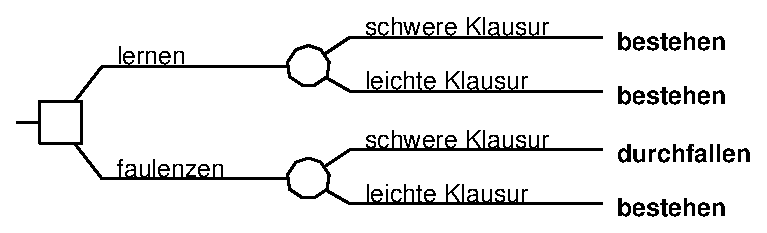
\includegraphics[width=8cm]{Grafiken/Beispiel1_1.eps}
\end{center}
Würde man diesen Entscheidungsbaum nach unserem "`mechanischen"' Verfahren in
eine Tabelle überführen, dann würden in den Spaltenüberschriften die Ereignisse
"`schwere Klausur \& schwere Klausur"', "`schwere Klausur \& leichte Klausur"',
"`leichte Klausur \& schwere Klausur"' und "`leichte Klausur \& leichte
Klausur"' stehen. Das hängt damit zusammen, dass der Algorithmus zunächst keine
Informationen darüber hat, ob unterschiedliche Zufallsknoten möglicherweise
identische Zufallsereignisse repräsentieren. Man müsste den
Entscheidungsbaum um entsprechende Informationen ergänzen (z.B. indem man eine
Verbindungslinie zwischen identischen Ereignissen zieht) und den Algorithmus so
anpassen, dass er unmögliche Ereigniskombinationen ("`schwere \& leichte
Klausur"') streicht. 

Weiterhin haben wir den Algorithmus zur Übersetzung von Bäumen in Tabellen
zunächst nur für {\em Binär-}bäume (d.h. Bäume, die an jeder Verzweigung nur
zwei Äste haben) beschrieben. Das ist aber unproblematisch, da man jeden
Entscheidungsbaum in einen binären Entscheidungsbaum umwandeln kann. Z.B. kann
der Entscheidungsbaum
\begin{center}
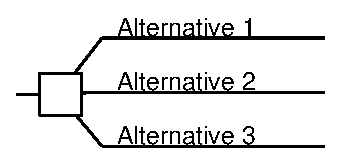
\includegraphics[width=5cm]{Grafiken/Beispiel1b_5.eps}
\end{center}
einfach in den Baum
\begin{center}
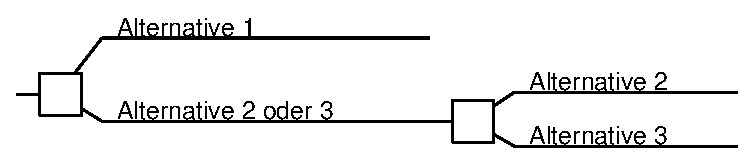
\includegraphics[width=10cm]{Grafiken/Beispiel1b_6.eps}
\end{center}
umgewandelt werden. Eine andere Alternative bestünde darin, den Algorithmus so
anzupassen, dass er sich auch für nicht binäre Entscheidungsbäume eignet
(siehe  Übungsaufgabe \ref{Algorithmusaufgabe} auf Seite
\pageref{Algorithmusaufgabe}).


\subsection{Literaturhinweise}

Zum Schluss ein par Worte zu der Fachliteratur, auf die sich diese Vorlesung
stützt, und die ich als Ergänzung zu diesem Skript als Begeleittexte empfehle:
Zum überwiegenden Teil werde ich in dieser Vorlesung dem Buch "`Choices. An
Introduction to Decision Theory"' von Micheal D. \cite{resnik:1987} folgen. Es
handelt sich dabei um eine didaktisch gut aufbereitete und sehr verständliche
Einführung in die Entscheidungstheorie und die Grundlagen der Spieltheorie.
% Speziell für die Spieltheorie wird auch die Einführung von Martin J. Osborne
% "`An Introduction to Game Theory" \cite{osborne:2004} verwendet.
Für die etwas mathematischeren Teile dieser Vorlesung, insbesondere für den
"`Satz von Arrow"' und die "`Neumann-Morgensternschen Nutzenfunktionen"', möchte
ich auch auf die sehr klare und verständliche Darstellung in dem Lehrbuch von
\cite{mascolell-whinston-green:1995} verweisen. Speziell was die philosophischen
Probleme im Zusammenhang mit der Entscheidungstheorie angeht, werde ich weiterhin
Das Buch von Mark Kaplan "`Decision Theory as Philosophy"' \cite[]{kaplan:1996}
hinzuziehen. Für die Themen aus dem Bereich Social Choice und Public Choicde, 
greife ich unter anderem auf Dennis C. Mueller: "`Public Choice III"'
\cite[]{mueller:2003} zurück. (Als kritische Ergänzung zu der sehr einseitigen
Darstellung Muellers ist, wie bereits erwähnt, das Buch "`The Pathologies of
Rational Choice"' von \cite{green-shapiro:1994}
sehr empfehlenswert.) Soweit in der Vorlesung auch wissenschaftstheoretische Fragen
berührt werden, beziehe ich mich hauptsächlich auf Gerhard Schurz' "`Einführung
in die Wissenschaftstheorie"' \cite[]{schurz:2006}.

